%
% laplace.tex
%
% (c) 2021 Prof Dr Andreas Müller, OST Ostschweizer Fachhochschule
%
\bgroup
\definecolor{darkgreen}{rgb}{0,0.6,0}
\begin{frame}[t]
\setlength{\abovedisplayskip}{5pt}
\setlength{\belowdisplayskip}{5pt}
\frametitle{Laplace-Matrix}
\vspace{-20pt}
\begin{columns}[t,onlytextwidth]
\begin{column}{0.48\textwidth}
\begin{center}
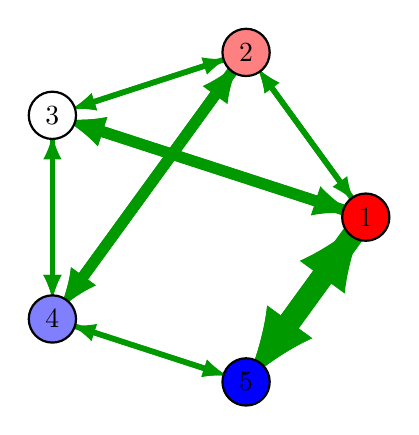
\begin{tikzpicture}[>=latex,thick]

\def\r{2.2}

\coordinate (A) at ({\r*cos(0*72)},{\r*sin(0*72)});
\coordinate (B) at ({\r*cos(1*72)},{\r*sin(1*72)});
\coordinate (C) at ({\r*cos(2*72)},{\r*sin(2*72)});
\coordinate (D) at ({\r*cos(3*72)},{\r*sin(3*72)});
\coordinate (E) at ({\r*cos(4*72)},{\r*sin(4*72)});

\draw[shorten >= 0.3cm,shorten <= 0.3cm] (A) -- (C);
\draw[color=white,line width=5pt] (B) -- (D);
\draw[shorten >= 0.3cm,shorten <= 0.3cm] (B) -- (D);

\draw[shorten >= 0.3cm,shorten <= 0.3cm] (A) -- (B);
\draw[shorten >= 0.3cm,shorten <= 0.3cm] (B) -- (C);
\draw[shorten >= 0.3cm,shorten <= 0.3cm] (C) -- (D);
\draw[shorten >= 0.3cm,shorten <= 0.3cm] (D) -- (E);
\draw[shorten >= 0.3cm,shorten <= 0.3cm] (E) -- (A);

\uncover<2-4>{
\draw[->,color=darkgreen,line width=2pt,shorten <= 0.25cm,shorten >= 0.25cm]
	(A) -- (B);
}

\uncover<3-7>{
\draw[->,color=darkgreen,line width=4pt,shorten <= 0.25cm,shorten >= 0.15cm]
	(A) -- (C);
}

\uncover<4-13>{
\draw[->,color=darkgreen,line width=8pt,shorten <= 0.25cm,shorten >= 0cm]
	(A) -- (E);
}

\uncover<5->{
\draw[<->,color=darkgreen,line width=2pt,shorten <= 0.25cm,shorten >= 0.25cm]
	(A) -- (B);
}

\uncover<6-8>{
\draw[->,color=darkgreen,line width=2pt,shorten <= 0.25cm,shorten >= 0.25cm]
	(B) -- (C);
}

\uncover<7-10>{
\draw[->,color=darkgreen,line width=4pt,shorten <= 0.25cm,shorten >= 0.15cm]
	(B) -- (D);
}

\uncover<8->{
\draw[<->,color=darkgreen,line width=4pt,shorten <= 0.15cm,shorten >= 0.15cm]
	(A) -- (C);
}

\uncover<9->{
\draw[<->,color=darkgreen,line width=2pt,shorten <= 0.25cm,shorten >= 0.25cm]
	(B) -- (C);
}

\uncover<10-11>{
\draw[->,color=darkgreen,line width=2pt,shorten <= 0.25cm,shorten >= 0.25cm]
	(C) -- (D);
}

\uncover<11->{
\draw[<->,color=darkgreen,line width=4pt,shorten <= 0.15cm,shorten >= 0.15cm]
	(B) -- (D);
}

\uncover<12->{
\draw[<->,color=darkgreen,line width=2pt,shorten <= 0.25cm,shorten >= 0.25cm]
	(C) -- (D);
}

\uncover<13-14>{
\draw[->,color=darkgreen,line width=2pt,shorten <= 0.25cm,shorten >= 0.25cm]
	(D) -- (E);
}

\uncover<14->{
\draw[<->,color=darkgreen,line width=8pt,shorten <= 0cm,shorten >= 0cm]
	(A) -- (E);
}

\uncover<15->{
\draw[<->,color=darkgreen,line width=2pt,shorten <= 0.25cm,shorten >= 0.25cm]
	(D) -- (E);
}

\fill[color=red] (A) circle[radius=0.3];
\fill[color=red!50] (B) circle[radius=0.3];
\fill[color=white] (C) circle[radius=0.3];
\fill[color=blue!50] (D) circle[radius=0.3];
\fill[color=blue] (E) circle[radius=0.3];

\draw (A) circle[radius=0.3];
\draw (B) circle[radius=0.3];
\draw (C) circle[radius=0.3];
\draw (D) circle[radius=0.3];
\draw (E) circle[radius=0.3];

\node at (A) {$1$};
\node at (B) {$2$};
\node at (C) {$3$};
\node at (D) {$4$};
\node at (E) {$5$};

\end{tikzpicture}
\end{center}
\uncover<16->{%
\begin{block}{Definition}
Laplace-Matrix
\[
L(G) = D(G) - A(G)
\]
\end{block}}
\end{column}
\begin{column}{0.48\textwidth}
\begin{align*}
f
&=
\begin{pmatrix}
f(1)\\
f(2)\\
f(3)\\
f(4)\\
f(5)
\end{pmatrix}
\\
\frac{df}{dt}
&=
-\kappa
\begin{pmatrix*}[r]
\only<1>{\phantom{-0}}
	\only<2>{\phantom{-}1}
	\only<3>{\phantom{-}2}
	\only<4->{\phantom{-}3}
	&\only<1>{\phantom{-0}}\only<2->{{-1}}%
	&\only<-2>{\phantom{-0}}\only<3->{{-1}}%
	&\uncover<16->{ 0}
	&\only<-3>{\phantom{-0}}\only<4->{{-1}}\\
\only<-4>{\phantom{-0}}\only<5->{{-1}}
	&\only<-4>{\phantom{-0}}
	\only<5>{\phantom{-}1}
	\only<6>{\phantom{-}2}
	\only<7->{\phantom{-}3}
	&\only<-5>{\phantom{-0}}\only<6->{{-1}}
	&\only<-6>{\phantom{-0}}\only<7->{{-1}}
	&\uncover<16->{ 0}\\
\only<-7>{\phantom{-0}}\only<8->{{-1}}
	&\only<-8>{\phantom{-0}}\only<9->{{-1}}
	&\only<-7>{\phantom{-0}}
	\only<8>{\phantom{-}1}
	\only<9>{\phantom{-}2}
	\only<10->{\phantom{-}3}
	&\only<-9>{\phantom{-0}}\only<10->{{-1}}
	&\uncover<16->{ 0}\\
\uncover<16->{ 0}
	&\only<-10>{\phantom{-0}}\only<11->{{-1}}
	&\only<-11>{\phantom{-0}}\only<12->{{-1}}
	&\only<-10>{\phantom{-0}}
	\only<11>{\phantom{-}1}
	\only<12>{\phantom{-}2}
	\only<13->{\phantom{-}3}
	&\only<-12>{\phantom{-0}}\only<13->{{-1}}\\
\only<-13>{\phantom{-0}}\only<14->{{-1}}
	&\uncover<16->{ 0}
	&\uncover<16->{ 0}
	&\only<-14>{\phantom{-0}}\only<15->{{-1}}
	&\only<-13>{\phantom{-0}}
	\only<14>{\phantom{-}1}
	\only<15->{\phantom{-}2}
\end{pmatrix*}
\begin{pmatrix}
f(1)\\
f(2)\\
f(3)\\
f(4)\\
f(5)
\end{pmatrix}
\\
\uncover<17->{
&=
-\kappa L f}
\end{align*}
\vspace{-20pt}
\uncover<18->{%
\begin{block}{Rekonstruktion}
Der Graph lässt sich aus $L$ rekonstruieren
\end{block}}
\end{column}
\end{columns}
\end{frame}

\egroup


